\documentclass[11pt,oneside]{report}

\usepackage[margin=1in,headheight=15pt]{geometry}
\usepackage[T1]{fontenc}
\usepackage[utf8]{inputenc}
\usepackage{lmodern}
\usepackage{microtype}
\usepackage{parskip}
\usepackage{amsmath}
\usepackage{booktabs}
\usepackage{longtable}
\usepackage{tabularx}
\usepackage{array}
\usepackage{enumitem}
\usepackage{xcolor}
\usepackage{listings}
\usepackage{graphicx}
\usepackage{fancyhdr}
\usepackage{lastpage}
\usepackage{hyperref}
\usepackage[most]{tcolorbox}
\usepackage{tikz}
\usetikzlibrary{arrows.meta,positioning,shapes.geometric,fit}

\definecolor{FracBlue}{HTML}{235789}
\definecolor{FracBlueLight}{HTML}{EAF1F8}
\definecolor{FracTeal}{HTML}{2A7F85}
\definecolor{FracGold}{HTML}{D9A441}
\definecolor{FracGray}{HTML}{4A5560}
\definecolor{CodeBg}{HTML}{F6F8FA}
\definecolor{CodeFrame}{HTML}{D9E0E6}
\definecolor{WarnBg}{HTML}{FFF7E8}
\definecolor{TipBg}{HTML}{EDF8F1}

\hypersetup{
  colorlinks=true,
  linkcolor=FracBlue,
  urlcolor=FracTeal,
  citecolor=FracBlue,
  pdftitle={FracVAL-Qt 1.0 User and Developer Guide},
  pdfauthor={FracVAL-Qt project documentation}
}

\pagestyle{fancy}
\fancyhf{}
\lhead{FracVAL-Qt 1.0}
\rhead{User and Developer Guide}
\cfoot{\thepage\ of \pageref{LastPage}}
\renewcommand{\headrulewidth}{0.4pt}

\setcounter{tocdepth}{2}
\setcounter{secnumdepth}{3}
\renewcommand{\arraystretch}{1.18}

\lstdefinestyle{fracval}{
  backgroundcolor=\color{CodeBg},
  basicstyle=\ttfamily\small,
  frame=single,
  rulecolor=\color{CodeFrame},
  breaklines=true,
  breakatwhitespace=false,
  showstringspaces=false,
  columns=fullflexible,
  keepspaces=true,
  tabsize=4,
  numbers=none,
  aboveskip=0.8em,
  belowskip=0.8em
}
\lstset{style=fracval}

\newtcolorbox{importantbox}{
  colback=FracBlueLight,
  colframe=FracBlue,
  title=Important,
  fonttitle=\bfseries,
  boxrule=0.8pt,
  arc=2mm
}
\newtcolorbox{tipbox}{
  colback=TipBg,
  colframe=FracTeal,
  title=Recommended practice,
  fonttitle=\bfseries,
  boxrule=0.8pt,
  arc=2mm
}
\newtcolorbox{warningbox}{
  colback=WarnBg,
  colframe=FracGold,
  title=Scientific / numerical caution,
  fonttitle=\bfseries,
  boxrule=0.8pt,
  arc=2mm
}

\newcommand{\FracVAL}{\textsc{FracVAL}}
\newcommand{\code}[1]{\texttt{#1}}

\begin{document}
\hypersetup{pageanchor=false}

\begin{titlepage}
  \centering
  \vspace*{1.2cm}
  {\color{FracBlue}\rule{\textwidth}{1.5pt}}\\[1.2cm]
  {\Huge\bfseries FracVAL-Qt 1.0\\[0.25cm]}
  {\LARGE User and Developer Guide\\[0.55cm]}
  {\large Fortran fractal aggregate engine, Python API, and native Qt desktop GUI}
  \\[1.2cm]

  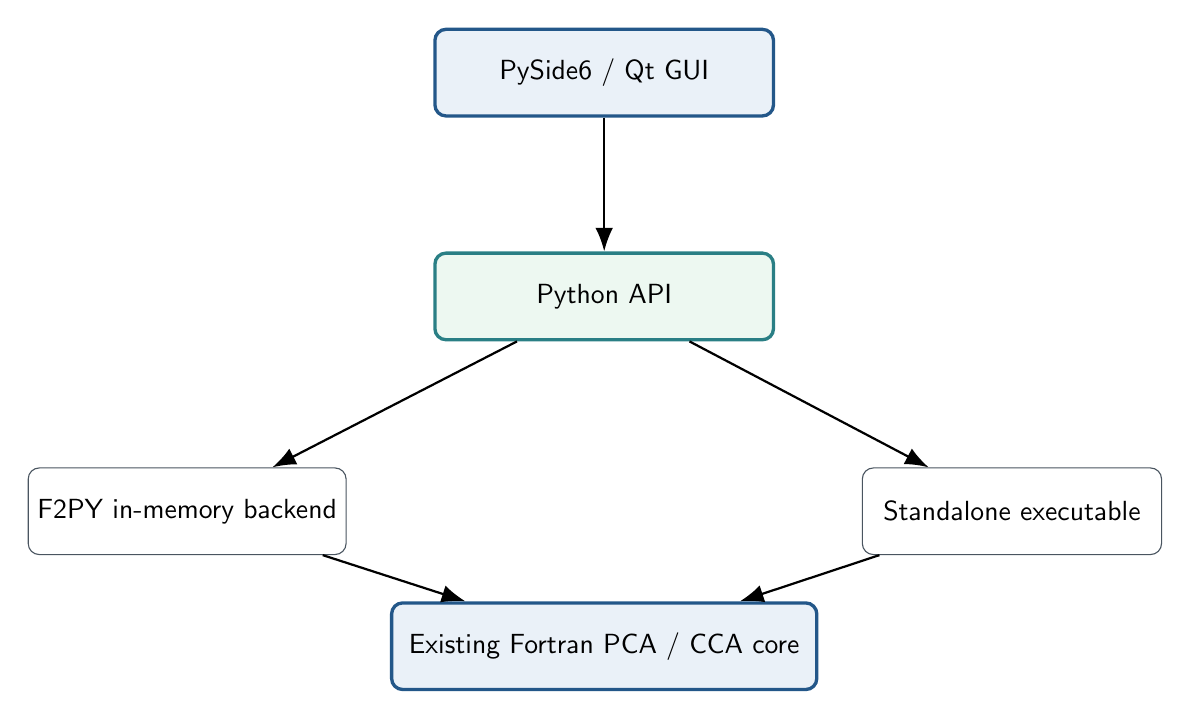
\begin{tikzpicture}[node distance=1.7cm, every node/.style={font=\sffamily}]
    \node[draw=FracBlue, very thick, rounded corners, fill=FracBlueLight, minimum width=4.3cm, minimum height=1.1cm] (gui) {PySide6 / Qt GUI};
    \node[draw=FracTeal, very thick, rounded corners, fill=TipBg, below=of gui, minimum width=4.3cm, minimum height=1.1cm] (api) {Python API};
    \node[draw=FracGray, rounded corners, below left=1.6cm and 1.1cm of api, minimum width=3.8cm, minimum height=1.1cm] (f2py) {F2PY in-memory backend};
    \node[draw=FracGray, rounded corners, below right=1.6cm and 1.1cm of api, minimum width=3.8cm, minimum height=1.1cm] (exe) {Standalone executable};
    \node[draw=FracBlue, very thick, rounded corners, fill=FracBlueLight, below=3.3cm of api, minimum width=5.4cm, minimum height=1.1cm] (core) {Existing Fortran PCA / CCA core};
    \draw[-{Latex[length=3mm]}, thick] (gui) -- (api);
    \draw[-{Latex[length=3mm]}, thick] (api) -- (f2py);
    \draw[-{Latex[length=3mm]}, thick] (api) -- (exe);
    \draw[-{Latex[length=3mm]}, thick] (f2py) -- (core);
    \draw[-{Latex[length=3mm]}, thick] (exe) -- (core);
  \end{tikzpicture}

  \vfill
  \begin{minipage}{0.88\textwidth}
  \small
  FracVAL-Qt preserves the established FracVAL numerical aggregation routines
  and adds runtime configuration, reproducible random seeds, a Python
  interface, an optional intended-contact overlap model, a native desktop GUI,
  3-D visualization, result export, and regression tests.

  The original FracVAL software and methodology were developed by J. Morán,
  A. Fuentes, F. Liu, and J. Yon. FracVAL-Qt is a GPLv3 derivative and does not
  imply endorsement of later modifications by the original authors.
  \end{minipage}
  \\[1.2cm]
  {\color{FracBlue}\rule{\textwidth}{1.5pt}}\\[0.5cm]
  {\small Documentation release: 1.0.0}
\end{titlepage}

\pagenumbering{roman}
\tableofcontents
\clearpage
\pagenumbering{arabic}
\hypersetup{pageanchor=true}

\chapter{What FracVAL Is and Which Interface to Use}

\FracVAL{} generates aggregates composed of spherical primary particles. The
numerical core uses particle-cluster aggregation (PCA) and cluster-cluster
aggregation (CCA) routines. In this distribution, those Fortran routines remain
the scientific engine while configuration, scripting, visualization, and
interactive use are handled by separate layers.

The main design goal is that changing a simulation parameter does \emph{not}
require recompiling the Fortran code. Recompilation is only necessary after
source-code changes or when building the native Python extension for a new
Python/platform environment.

\section{Origin, attribution, citation, and license}

FracVAL-Qt is a derivative and modernization of the original \FracVAL{}
Fortran software developed by J. Morán, A. Fuentes, F. Liu, and J. Yon. The
original scientific work is:

\begin{quote}
J. Morán, A. Fuentes, F. Liu, and J. Yon, ``FracVAL: An improved tunable
algorithm of cluster-cluster aggregation for generation of fractal structures
formed by polydisperse primary particles,'' \emph{Computer Physics
Communications}, 239 (2019), 225--237. DOI:
\href{https://doi.org/10.1016/j.cpc.2019.01.015}{10.1016/j.cpc.2019.01.015}.
\end{quote}

The corresponding original software/data release is archived at Mendeley Data,
Version 1, DOI:
\href{https://doi.org/10.17632/mgf8wdcsfb.1}{10.17632/mgf8wdcsfb.1}.
The original release specifies the GNU General Public License version 3. This
repository therefore includes the GPLv3 text in \path{LICENSE} and keeps a
plain-language provenance record in \path{NOTICE.md}.

The original authors should be credited for the original FracVAL algorithm and
Fortran implementation. Runtime configuration, the Python/F2PY layer, Qt GUI,
visualization, testing infrastructure, reproducibility controls, and overlap
extensions described in this manual are subsequent modifications maintained in
FracVAL-Qt. Nothing in this distribution implies that the original authors
created or endorsed those later changes.

For publications, cite the original Morán et al. paper for the FracVAL
methodology. When exact software provenance matters, additionally cite the
FracVAL-Qt repository and release/tag used. Machine-readable citation metadata
is provided in \path{CITATION.cff}; a copy-pasteable BibTeX entry is in
\path{CITATION.md}.

\begin{importantbox}
Do not remove original authorship or license notices when redistributing a
modified version. FracVAL-Qt is distributed under GPLv3; see \path{LICENSE} for
the complete terms.
\end{importantbox}

\section{Three supported workflows}

\begin{longtable}{>{\bfseries}p{0.16\textwidth}p{0.34\textwidth}p{0.40\textwidth}}
\toprule
Interface & Use it when & Typical entry point \\
\midrule
Qt GUI & You want to interactively change parameters, generate one or many aggregates, inspect them in 3-D, change appearance, and export results. & \code{fracval-gui} \\
Python API & You are writing scripts, notebooks, parameter sweeps, optimization loops, pipelines, or another application. & \code{from fracval import FracVALConfig, generate} \\
Fortran CLI & You want a small compiled executable controlled by a namelist file, for example on a compute node. & \code{./build/fracval fracval.in} \\
\bottomrule
\end{longtable}

\begin{tipbox}
For new Python-based scientific work, use the public Python API even if you also
use the supplied GUI. Do not make your analysis code depend on GUI widgets.
This keeps generation reproducible and makes your workflow easier to test.
\end{tipbox}

\section{What changed relative to the legacy source layout}

The modernization in this package includes:
\begin{itemize}[leftmargin=1.6em]
  \item runtime input instead of compile-time user parameters;
  \item out-of-tree Fortran compilation under \path{build/};
  \item deterministic random-seed control;
  \item an F2PY wrapper that returns particle arrays directly to Python;
  \item a native PySide6 / Qt desktop interface;
  \item offline Plotly 3-D visualization embedded in the GUI;
  \item fixed or bounded statistical overlap at intended joining contacts;
  \item contact-overlap history and derived geometry in Python;
  \item portable JSON configuration and result-bundle helpers;
  \item deterministic mono/polydisperse and overlap regression tests.
\end{itemize}

\chapter{Project Structure}

The source tree is intentionally layered so that the GUI, Python API, and
Fortran engine can evolve independently.

\begin{lstlisting}
FracVAL-Qt/
|-- Makefile
|-- pyproject.toml
|-- fracval.in
|-- README.md
|-- CHANGELOG.md
|-- LICENSE
|-- NOTICE.md
|-- CITATION.cff
|-- CITATION.md
|-- CONTRIBUTING.md
|-- GITHUB_SETUP.md
|-- src/                       # Fortran source
|   |-- Ctes.f90
|   |-- Frac_VAL_CCA.f90
|   |-- CCA_module.f90
|   |-- PCA_Subclusters_module.f90
|   |-- PCA_cca.f90
|   |-- a_Random_PP.f90
|   |-- RAND_SAMPLE.f90
|   |-- random.f90
|   |-- Save_results_CC.f90
|   `-- fracval_python_api.f90
|-- python/
|   |-- build_fortran_extension.py
|   `-- fracval/
|       |-- config.py
|       |-- aggregate.py
|       |-- engine.py
|       |-- io.py
|       |-- visualization.py
|       |-- diagnostics.py
|       `-- desktop/
|-- gui/                       # source-tree GUI launcher
|-- examples/                  # Python integration examples
|-- tests/                     # Fortran, Python, Qt and model tests
|-- plot/                      # standalone plots and notebooks
|-- doc/                       # this manual and quick references
|-- results/                   # default CLI output
`-- build/                     # generated native/doc build products
\end{lstlisting}

\section{Source directories}

\subsection{\texttt{src/}: scientific engine}

\path{src/} contains the Fortran aggregation implementation. The modernized
runtime state and namelist parsing live in \path{Ctes.f90}. The thin wrapper
\path{fracval_python_api.f90} exposes a single aggregate-generation routine to
F2PY without moving the PCA/CCA algorithm into Python.

\subsection{\texttt{python/fracval/}: public Python library}

This directory is the normal integration boundary for Python users:
\begin{description}[leftmargin=3.1cm,style=nextline]
  \item[\path{config.py}] immutable validated runtime configuration;
  \item[\path{engine.py}] backend selection and single/batch generation;
  \item[\path{aggregate.py}] aggregate result container and derived geometry;
  \item[\path{io.py}] native data reading and portable result bundles;
  \item[\path{visualization.py}] reusable Plotly/Matplotlib visualization;
  \item[\path{diagnostics.py}] environment and backend diagnostics;
  \item[\path{desktop/}] Qt-specific application code.
\end{description}

\subsection{\texttt{python/fracval/desktop/}: native GUI}

The desktop package contains the Qt main window, background worker, WebEngine
viewer, and Qt plugin-path setup. Scientific generation is not implemented in
these modules; the GUI calls the same public Python engine used by scripts.

\section{Generated directories}

Compiler products belong under \path{build/}. A platform-specific F2PY module
is generated under \path{python/fracval/} and removed by \code{make clean}.
The source ZIP intentionally does not carry a Linux or macOS binary extension,
because native extensions must match the user's Python version and machine.

\chapter{Installation and First Build}

\section{Requirements}

Core generation needs:
\begin{itemize}
  \item Python 3.10 or newer for the Python API;
  \item NumPy;
  \item GNU Fortran (\code{gfortran});
  \item a C compiler for the F2PY wrapper;
  \item GNU Make for the supplied build commands.
\end{itemize}

The native GUI additionally needs PySide6. Plotly is a base Python dependency
because it is used by the GUI viewer and public interactive plotting API.
Static Matplotlib plotting and notebooks are available through the optional
\code{plot} dependency group.

\section{macOS}

Install GNU Fortran with Homebrew if it is not already available:

\begin{lstlisting}[language=bash]
brew install gcc
\end{lstlisting}

Then, from the project root:

\begin{lstlisting}[language=bash]
python3 -m venv .venv
source .venv/bin/activate
python -m pip install --upgrade pip
make install-gui PYTHON=python
make
make qt-check PYTHON=python
make gui-test PYTHON=python
make test PYTHON=python
\end{lstlisting}

\begin{importantbox}
The virtual environment matters on macOS, particularly when Conda, Homebrew,
and system Python installations coexist. After activation, verify
\code{which python}. The same Python interpreter should be used for installing
PySide6, building the F2PY extension, and launching the GUI.
\end{importantbox}

\section{Linux}

On Debian/Ubuntu-like systems, the native prerequisites are typically:

\begin{lstlisting}[language=bash]
sudo apt install gfortran make gcc
\end{lstlisting}

Then use the same virtual-environment and \code{make install-gui} sequence as
on macOS.

\section{Windows}

The most predictable Fortran workflow is WSL/WSL2 using the Linux instructions.
A native Windows build may be possible with a compatible MinGW/MSYS2 Fortran
and C toolchain, but this source package is primarily structured and tested
around POSIX-style build commands. Native Qt/PySide6 itself is cross-platform,
but the F2PY native-link step must match the selected compiler and Python ABI.

\section{Installation targets}

\begin{longtable}{p{0.29\textwidth}p{0.61\textwidth}}
\toprule
Command & Purpose \\
\midrule
\code{make install PYTHON=python} & Editable Python package installation plus local F2PY extension build. \\
\code{make install-gui PYTHON=python} & Same, with PySide6 GUI dependencies. \\
\code{make} & Build the standalone Fortran executable at \path{build/fracval}. \\
\code{make python-ext PYTHON=python} & Rebuild only the in-memory F2PY extension. \\
\code{make clean} & Remove native compiler products and extension binaries. \\
\bottomrule
\end{longtable}

\section{Verify the installation}

Run:

\begin{lstlisting}[language=bash]
fracval-info
\end{lstlisting}

A healthy installation should report the active Python, package directory, and
at least one available backend. For the preferred Python workflow you want:

\begin{lstlisting}
F2PY extension      : available
Available backends  : extension, executable
\end{lstlisting}

For GUI-specific diagnostics:

\begin{lstlisting}[language=bash]
fracval-qt-check
\end{lstlisting}

On macOS, the available platform plugins should include \code{cocoa}. The
launcher explicitly configures Qt's platform-plugin path before constructing
\code{QApplication} to avoid the common empty-plugin-path failure.

\chapter{Five-Minute Workflows}

\section{Launch the GUI}

After the first build:

\begin{lstlisting}[language=bash]
cd /path/to/FracVAL-Qt
source .venv/bin/activate
fracval-gui
\end{lstlisting}

You do not run \code{make} again merely because \code{N}, \code{Df}, \code{kf},
particle size, overlap, or aggregate count changed.

\section{Generate from Python}

\begin{lstlisting}[language=Python]
from fracval import FracVALConfig, generate

config = FracVALConfig(
    n=100,
    df=1.79,
    kf=1.40,
    rp_g=15.0,
    rp_gstd=1.0,
    seed=12345,
)

aggregate = generate(config)
print(aggregate.data.shape)
print(aggregate.radius_of_gyration)
\end{lstlisting}

\section{Run the standalone executable}

\begin{lstlisting}[language=bash]
make
./build/fracval fracval.in
\end{lstlisting}

Edit \path{fracval.in} and rerun the same executable. No recompilation is
needed for runtime parameter changes.

\chapter{Native Qt GUI Guide}

\section{Window organization}

The desktop application uses a scrollable control panel on the left and an
interactive 3-D viewer on the right. The layout can be resized with the
splitter.

\begin{center}
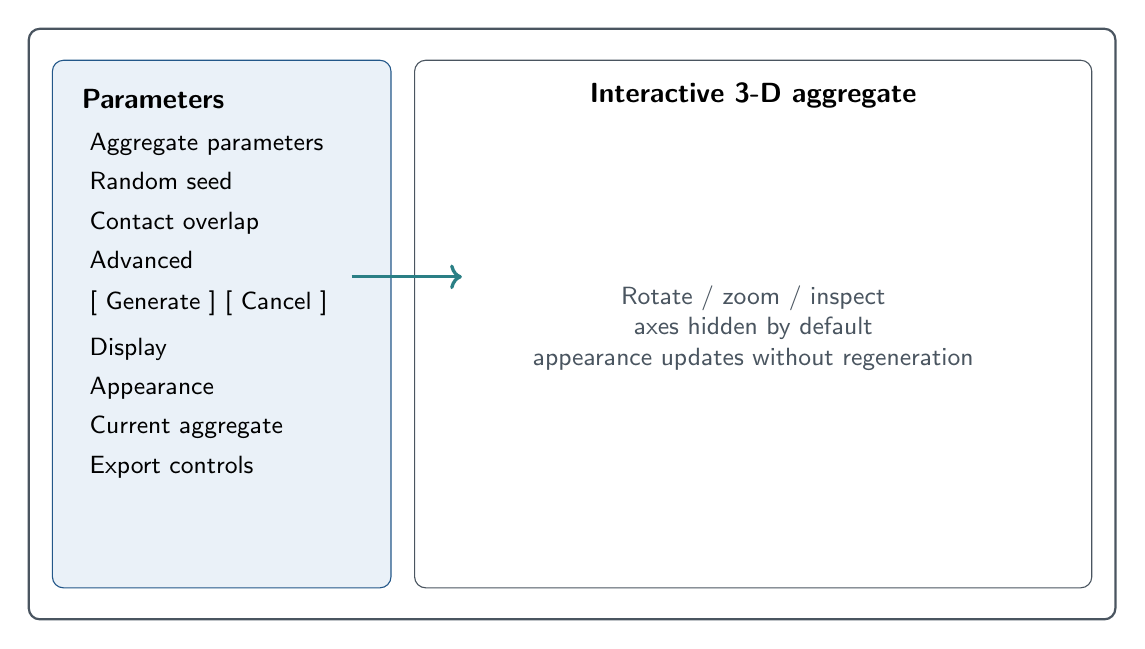
\begin{tikzpicture}[font=\sffamily\small]
  \draw[rounded corners, thick, color=FracGray] (0,0) rectangle (13.8,7.5);
  \draw[fill=FracBlueLight, draw=FracBlue, rounded corners] (0.3,0.4) rectangle (4.6,7.1);
  \draw[fill=white, draw=FracGray, rounded corners] (4.9,0.4) rectangle (13.5,7.1);
  \node[anchor=north west, font=\bfseries\sffamily] at (0.55,6.85) {Parameters};
  \node[anchor=north west] at (0.65,6.3) {Aggregate parameters};
  \node[anchor=north west] at (0.65,5.8) {Random seed};
  \node[anchor=north west] at (0.65,5.3) {Contact overlap};
  \node[anchor=north west] at (0.65,4.8) {Advanced};
  \node[anchor=north west] at (0.65,4.3) {[ Generate ] [ Cancel ]};
  \node[anchor=north west] at (0.65,3.7) {Display};
  \node[anchor=north west] at (0.65,3.2) {Appearance};
  \node[anchor=north west] at (0.65,2.7) {Current aggregate};
  \node[anchor=north west] at (0.65,2.2) {Export controls};
  \node[font=\bfseries\sffamily] at (9.2,6.65) {Interactive 3-D aggregate};
  \node[align=center, text=FracGray] at (9.2,3.7) {Rotate / zoom / inspect\\axes hidden by default\\appearance updates without regeneration};
  \draw[->, very thick, color=FracTeal] (4.1,4.35) -- (5.5,4.35);
\end{tikzpicture}
\end{center}

\section{Aggregate parameters}

\begin{description}[style=nextline,leftmargin=3.7cm]
  \item[Primary particles (N)] Number of spheres in each aggregate.
  \item[Fractal dimension (Df)] Fractal dimension used by the legacy target-radius relation.
  \item[Fractal prefactor (kf)] Fractal prefactor used with \code{Df}.
  \item[Particle distribution] Monodisperse or polydisperse.
  \item[Geometric mean radius] \code{rp\_g}, in the user's chosen length units.
  \item[Geometric radius std. dev.] \code{rp\_gstd}. The GUI forces 1.0 in monodisperse mode.
  \item[Number of aggregates] Number generated in the current batch.
\end{description}

All coordinates and radii use the same arbitrary length unit. If \code{rp\_g}
is interpreted in nanometers, the returned coordinates are also in nanometers.
The engine does not attach a unit string.

\section{Random seeds}

With \emph{Use fixed base seed} enabled, the entered base seed makes a single
run reproducible and gives a deterministic sequence of per-aggregate seeds for
a batch. Disable it for exploratory random generation. The GUI always displays
the actual seed stored in each returned aggregate.

\begin{tipbox}
For publication-quality or archived simulation work, use fixed seeds and export
JSON metadata or result bundles. The seed should be treated as part of the
simulation input.
\end{tipbox}

\section{Contact overlap}

The GUI exposes three modes:
\begin{itemize}
  \item \textbf{None (touching)}: legacy contact behavior;
  \item \textbf{Fixed}: every intended joining contact uses one overlap fraction;
  \item \textbf{Statistical}: each intended contact samples a bounded normal distribution.
\end{itemize}

The GUI displays overlap values as percentages. The Python API and Fortran
namelist use fractions, so 5 percent in the GUI corresponds to \code{0.05} in
Python.

Unrelated particle pairs are still protected by the strict unintended-overlap
tolerance. See Chapter~\ref{chap:overlap} for details.

\section{Advanced controls}

The Advanced panel contains:
\begin{itemize}
  \item \code{Ext\_case}, the legacy extreme-case switch;
  \item \code{Nsubcl\_perc}, sub-cluster fraction (normally 0.10);
  \item \code{tol\_ov}, numerical tolerance for unintended overlap;
  \item maximum construction attempts;
  \item backend selection (auto, extension, or executable when available).
\end{itemize}

Unless reproducing a legacy special case, keep \code{Ext\_case=0}. Do not use
\code{tol\_ov} as a physical overlap control; use the Contact overlap panel.

\section{Generation, progress, and cancellation}

Click \emph{Generate}. A Qt worker object performs generation outside the GUI
event loop. For batches, each completed aggregate is added to the selection box
and the progress bar advances.

Cancellation is cooperative \emph{between} aggregates. The legacy Fortran
routine cannot safely be interrupted in the middle of one aggregate build, so
clicking Cancel does not forcibly terminate the current native routine.

\section{Display and appearance}

The Display panel offers:
\begin{itemize}
  \item \textbf{Spheres}: geometric sphere meshes, best for smaller aggregates;
  \item \textbf{Centers}: lighter marker rendering for large aggregates;
  \item sphere resolution for the mesh mode.
\end{itemize}

The Appearance panel controls rendering only; it does not regenerate or modify
the physical aggregate. Controls include:
\begin{itemize}
  \item solid color or color by particle radius;
  \item particle color and Plotly color scale;
  \item opacity;
  \item shininess/specular appearance in sphere mode;
  \item background color;
  \item XYZ axes/grid visibility (off by default);
  \item radius legend and plot title visibility.
\end{itemize}

\section{Statistics}

For the selected aggregate the GUI shows particle count, seed, backend,
construction attempts (when reported), mean radius, contact count, overlap
statistics, radius of gyration, and bounding radius.

The Python radius of gyration includes the intrinsic moment contribution of
solid spheres (see Section~\ref{sec:derived}). This reported quantity is a
post-generation geometric metric and should not be confused blindly with the
intermediate target radius used inside the legacy placement routines.

\section{Saving and loading}

The File menu can save/load parameter JSON. A GUI parameter file includes:
\begin{itemize}
  \item the \code{FracVALConfig} fields;
  \item batch count;
  \item backend selection;
  \item viewer appearance.
\end{itemize}

The GUI exports the selected aggregate as DAT, CSV, contacts CSV, XYZ, metadata
JSON, or a standalone interactive HTML view. A whole batch can be written as a
ZIP archive.

\chapter{Python API}

\section{Import surface}

The supported public interface is exported from \code{fracval}:

\begin{lstlisting}[language=Python]
from fracval import (
    Aggregate,
    FracVALConfig,
    GenerationError,
    ViewerAppearance,
    generate,
    generate_batch,
    iter_generate_batch,
    load_data,
    save_bundle,
    load_bundle,
    plot_3d,
    plot_static,
    available_backends,
    extension_available,
    runtime_info,
)
\end{lstlisting}

Downstream code should prefer these names rather than importing private modules
or \path{fracval.desktop} internals.

\section{Configuration object}

\code{FracVALConfig} is an immutable dataclass. Calling \code{validate()} checks
physical/numerical ranges before invoking Fortran.

\begin{lstlisting}[language=Python]
from fracval import FracVALConfig

cfg = FracVALConfig(
    n=250,
    df=1.80,
    kf=1.20,
    rp_g=20.0,
    rp_gstd=1.5,
    seed=73001,
    max_attempts=500,
)
cfg.validate()
\end{lstlisting}

Because it is immutable, derive variants without mutating shared state:

\begin{lstlisting}[language=Python]
case_b = cfg.with_updates(df=1.9, kf=1.35)
case_c = cfg.with_seed(73002)
\end{lstlisting}

\subsection{Configuration JSON}

\begin{lstlisting}[language=Python]
cfg.save_json("case.json")
restored = FracVALConfig.load_json("case.json")
\end{lstlisting}

\code{load\_json()} also accepts the richer JSON file saved by the Qt GUI and
extracts its nested \code{config} object.

\section{Single aggregate generation}

\begin{lstlisting}[language=Python]
from fracval import generate

agg = generate(cfg, backend="auto")
\end{lstlisting}

\code{backend="auto"} prefers the F2PY extension and falls back to the
standalone executable if available. Use \code{extension} or \code{executable}
when a workflow requires one specifically.

\section{The Aggregate object}\label{sec:derived}

\code{Aggregate} contains NumPy arrays and provenance:

\begin{lstlisting}[language=Python]
agg.x                 # (N,)
agg.y
agg.z
agg.radius
agg.xyz               # (N, 3)
agg.data              # (N, 4): x, y, z, radius
agg.config
agg.seed
agg.backend
agg.attempts
\end{lstlisting}

The mass weighting used by geometric metrics is proportional to \(r^3\), so a
common material density cancels. The Python center of mass is

\begin{equation}
\mathbf{r}_{\mathrm{cm}} =
\frac{\sum_i r_i^3\,\mathbf{r}_i}{\sum_i r_i^3}.
\end{equation}

The reported radius of gyration includes the intrinsic moment of each solid
sphere:

\begin{equation}
R_g = \left[
\frac{\sum_i r_i^3\left(\lVert\mathbf{r}_i-\mathbf{r}_{\mathrm{cm}}\rVert^2
+ \frac{3}{5}r_i^2\right)}{\sum_i r_i^3}
\right]^{1/2}.
\end{equation}

The bounding radius is the maximum center distance from the aggregate center of
mass plus that particle's radius.

\section{Batch generation}

\begin{lstlisting}[language=Python]
from fracval import generate_batch

items = generate_batch(50, cfg)
\end{lstlisting}

For long runs, prefer the streaming form:

\begin{lstlisting}[language=Python]
from fracval import iter_generate_batch

for index, agg in enumerate(iter_generate_batch(50, cfg), start=1):
    print(index, agg.seed, agg.radius_of_gyration)
\end{lstlisting}

A deterministic NumPy random generator derives one seed per aggregate from the
resolved base seed. This makes the batch seed sequence repeatable.

\section{Result bundles}

Native \code{.dat} files are intentionally simple and contain only four columns.
For reproducible Python workflows, save metadata alongside particle data:

\begin{lstlisting}[language=Python]
from fracval import save_bundle, load_bundle

paths = save_bundle(agg, "results/case01", stem="aggregate_0001")
restored = load_bundle(paths["json"])
\end{lstlisting}

By default a bundle writes:
\begin{itemize}
  \item \code{aggregate\_0001.dat};
  \item \code{aggregate\_0001.csv};
  \item \code{aggregate\_0001.contacts.csv};
  \item \code{aggregate\_0001.json}.
\end{itemize}

Add XYZ when required:

\begin{lstlisting}[language=Python]
save_bundle(
    agg,
    "results/case01",
    stem="aggregate_0001",
    formats=("dat", "csv", "contacts", "xyz", "json"),
)
\end{lstlisting}

\begin{warningbox}
A bare DAT file cannot reconstruct \code{Df}, \code{kf}, seed, overlap model,
or backend. Use bundle metadata or another explicit provenance record for
scientific archival.
\end{warningbox}

\section{Interactive visualization}

\begin{lstlisting}[language=Python]
from fracval import ViewerAppearance, plot_3d

appearance = ViewerAppearance(
    particle_color="#CC5500",
    opacity=0.85,
    shininess=0.70,
    background_color="#FFFFFF",
    show_axes=False,
)

fig = plot_3d(agg, mode="spheres", appearance=appearance)
fig.show()
\end{lstlisting}

Radius coloring:

\begin{lstlisting}[language=Python]
appearance = ViewerAppearance(
    color_mode="radius",
    colorscale="Plasma",
    show_colorbar=True,
    show_axes=False,
)
fig = plot_3d(agg, appearance=appearance)
\end{lstlisting}

For large \(N\), \code{mode="centers"} is substantially lighter than generating
sphere meshes.

\section{Error handling}

Configuration errors raise \code{ValueError}; generation failures raise
\code{GenerationError}:

\begin{lstlisting}[language=Python]
from fracval import GenerationError

try:
    agg = generate(cfg)
except (GenerationError, ValueError) as exc:
    print(f"FracVAL failed: {exc}")
\end{lstlisting}

Do not silently discard a generation failure in automated studies. Record the
case parameters, seed, and error so the failed region can be investigated.

\section{Diagnostics from Python}

\begin{lstlisting}[language=Python]
from fracval import format_runtime_info, runtime_info

print(format_runtime_info())
info = runtime_info()
\end{lstlisting}

This is useful when embedding FracVAL in another application and collecting a
support report.

\chapter{Embedding FracVAL in Another Python Codebase}

\section{Recommended boundary}

Treat FracVAL as a generator service returning data, not as a GUI component:

\begin{lstlisting}
your_project/
|-- simulation.py  ---> fracval.FracVALConfig / fracval.generate
|-- analysis.py    ---> Aggregate or NumPy arrays
|-- database.py    ---> metadata / bundles
`-- ui.py          ---> your own UI, if any
\end{lstlisting}

A minimal wrapper is:

\lstinputlisting[language=Python,caption={Library-style integration example}]{../examples/python/06_embed_in_your_project.py}

\section{Why this boundary matters}

The Python API is stable enough to use from notebooks, command-line programs,
optimizers, and other desktop tools. In contrast, the Qt widget hierarchy is an
implementation detail of the supplied GUI and can change without affecting
scientific generation.

\section{Parallel workloads}

The legacy Fortran core stores runtime arrays and settings in module-global
state. The F2PY backend therefore protects calls with a Python lock. The wrapper
releases Python's GIL while Fortran executes, so the Qt event loop remains
responsive, but native generation calls are serialized within one process.

For genuine parallel parameter sweeps, use separate processes rather than
multiple Python threads. Each process has independent Fortran module state.
Validate scaling and reproducibility on the target system before launching very
large studies.

\section{Adding Python-only post-processing}

Analysis that does not affect construction should stay in Python. Example:

\begin{lstlisting}[language=Python]
import numpy as np


def radial_distances(aggregate):
    center = aggregate.center_of_mass
    return np.linalg.norm(aggregate.xyz - center, axis=1)
\end{lstlisting}

This avoids touching the native engine and makes unit testing simpler.

\chapter{Standalone Fortran Runtime Interface}

\section{The namelist file}

The executable reads a standard Fortran namelist at runtime. The default
\path{fracval.in} is structurally:

\begin{lstlisting}
&fracval
    N                   = 100
    Df                  = 1.79
    kf                  = 1.40
    rp_g                = 15.0
    rp_gstd             = 1.00
    Quantity_aggregates = 1
    Ext_case            = 0
    Nsubcl_perc         = 0.10
    tol_ov              = 1.0e-6
    random_seed_value   = -1
    overlap_mode        = 'none'
    overlap_fraction    = 0.05
    overlap_mean        = 0.05
    overlap_std         = 0.02
    overlap_max         = 0.12
    output_dir          = 'results'
/
\end{lstlisting}

The block starts with \code{\&fracval} and ends with \code{/}. Fortran namelist
names are case-insensitive. A relative output path is interpreted relative to
the directory from which the executable is launched.

\section{Input parameter reference}

\begin{longtable}{p{0.25\textwidth}p{0.43\textwidth}p{0.22\textwidth}}
\toprule
Parameter & Meaning & Validation / guidance \\
\midrule
\endhead
\code{N} & Primary particles per aggregate & integer, at least 5 \\
\code{Df} & Fractal dimension & positive \\
\code{kf} & Fractal prefactor & positive \\
\code{rp\_g} & Geometric mean primary-particle radius & positive \\
\code{rp\_gstd} & Geometric standard deviation & at least 1; 1 is monodisperse \\
\code{Quantity\_aggregates} & Number of successful aggregates to write & at least 1 \\
\code{Ext\_case} & Legacy extreme-case switch & 0 or 1; normally 0 \\
\code{Nsubcl\_perc} & Initial sub-cluster fraction & in (0,1]; normally 0.10 \\
\code{tol\_ov} & Unintended-overlap numerical tolerance & positive; normally \(10^{-6}\) \\
\code{random\_seed\_value} & Fortran random seed & -1 runtime default; nonnegative fixed seed \\
\code{overlap\_mode} & Intended contact overlap & none, fixed, statistical \\
\code{overlap\_fraction} & Fixed overlap fraction & 0 means touching \\
\code{overlap\_mean} & Statistical overlap mean & nonnegative fraction \\
\code{overlap\_std} & Statistical overlap std. dev. & nonnegative \\
\code{overlap\_max} & Statistical hard upper bound & in (0,0.95) \\
\code{output\_dir} & Output directory & quoted path; created automatically \\
\bottomrule
\end{longtable}

\section{Run multiple cases without recompilation}

\begin{lstlisting}[language=bash]
./build/fracval cases/monodisperse.in
./build/fracval cases/polydisperse.in
./build/fracval cases/overlap_05.in
\end{lstlisting}

This is the central runtime-interface improvement: all normal simulation
settings are read from the input file.

\chapter{Model and Numerical Behavior}

\section{Fractal target relation}

The legacy placement routines compute target gyration radii using the geometric
mean primary-particle radius and the fractal relation implemented in the source:

\begin{equation}
R_{g,\mathrm{target}} = r_{p,g}\left(\frac{N}{k_f}\right)^{1/D_f}.
\end{equation}

For polydisperse working sets, \(r_{p,g}\) is obtained from the geometric mean of
the radii currently being considered. This relation guides PCA/CCA placement;
the Python post-generation \path{Aggregate.radius_of_gyration} is an
independently calculated geometric metric of the final spheres.

\section{Primary-particle size distribution}

\code{rp\_gstd=1.0} produces equal radii (monodisperse). Values above one use
the lognormal primary-particle radius generator in the Fortran engine, centered
on the geometric mean \code{rp\_g}. Keep \code{rp\_g}, coordinates, and all
other lengths in one consistent unit system.

\section{Construction restarts}

For some stochastic configurations, a candidate PCA/CCA construction cannot be
continued without violating constraints. The generator then restarts. This is
normal behavior up to a point; repeated failure may indicate a difficult or
incompatible parameter combination.

The Python F2PY interface limits this using \code{max\_attempts}. The GUI exposes
the same control. A generation that exhausts the limit raises
\code{GenerationError} rather than hanging indefinitely.

\chapter{Intended Contact Overlap}\label{chap:overlap}

\section{Purpose}

The overlap feature is a controlled model extension. It is not implemented by
loosening global collision detection. Instead, it modifies only the selected
particle-particle contact used to join a monomer or cluster.

For particles with radii \(R_i\) and \(R_j\), touching contact has center
distance

\begin{equation}
d_{ij}=R_i+R_j.
\end{equation}

With intended overlap fraction \(\epsilon\), the joining distance is

\begin{equation}
d_{ij}=(R_i+R_j)(1-\epsilon).
\end{equation}

Thus \(\epsilon=0.05\) means a 5 percent reduction from touching separation,
independent of the absolute particle size.

\section{Fixed overlap}

Python:

\begin{lstlisting}[language=Python]
cfg = FracVALConfig(
    n=100,
    seed=12345,
    overlap_mode="fixed",
    overlap_fraction=0.05,
)
\end{lstlisting}

Fortran namelist:

\begin{lstlisting}
overlap_mode     = 'fixed'
overlap_fraction = 0.05
\end{lstlisting}

\section{Statistical overlap}

For each intended joining contact, a normal candidate centered at
\code{overlap\_mean} with standard deviation \code{overlap\_std} is sampled.
Values outside \([0,\,\code{overlap\_max}]\) are rejected and redrawn. Therefore
the realized contact distribution is a truncated/bounded distribution and its
sample mean need not equal the unbounded input mean exactly.

\begin{lstlisting}[language=Python]
cfg = FracVALConfig(
    n=100,
    seed=12345,
    overlap_mode="statistical",
    overlap_mean=0.05,
    overlap_std=0.02,
    overlap_max=0.12,
)
\end{lstlisting}

\section{Collision protection}

All other newly introduced pair intersections remain subject to \code{tol\_ov}.
This is critical: enabling 5 percent intended overlap does not permit every
particle pair in the aggregate to interpenetrate by 5 percent.

\section{Recorded contact history}

A successful tree-like aggregate normally contains \(N-1\) intended joining
contacts. The Python object exposes:

\begin{lstlisting}[language=Python]
agg.contact_overlaps
agg.contact_count
agg.mean_contact_overlap
agg.std_contact_overlap
agg.max_contact_overlap
\end{lstlisting}

The standalone executable writes a companion \code{.contacts.csv} file.
Currently the contact sidecar records construction order and overlap fraction,
not persistent final particle-pair IDs.

\begin{warningbox}
Overlap changes the particle-center geometry and can therefore change derived
morphology such as radius of gyration. Treat overlap settings as part of the
physical model, not merely a rendering choice. Large overlap can also increase
construction difficulty and restart frequency.
\end{warningbox}

\chapter{Output Formats and Provenance}

\section{Native DAT}

Each line contains:

\begin{lstlisting}
x  y  z  radius
\end{lstlisting}

There is no header, preserving compatibility with the legacy FracVAL data
format.

\section{CSV}

The Python/GUI CSV export adds a header:

\begin{lstlisting}
x,y,z,radius
\end{lstlisting}

\section{Contact CSV}

\begin{lstlisting}
contact_index,overlap_fraction
1,0.0471
2,0.0618
...
\end{lstlisting}

\section{XYZ}

The Python exporter uses a generic XYZ-like particle-center format with pseudo
atom label \code{P}. Radius is not part of standard XYZ coordinates, so use DAT
or CSV when particle size must be preserved.

\section{Metadata JSON}

\code{Aggregate.metadata()} includes the configuration, seed, attempts,
backend, derived geometry, and contact-overlap array. This is the preferred
machine-readable provenance record.

\section{Interactive HTML}

The GUI and Plotly helpers can export a self-contained interactive HTML view.
This is a visualization artifact, not the authoritative scientific data file.

\chapter{Visualization Tools}

\section{Standalone plotting script}

Plot a saved aggregate:

\begin{lstlisting}[language=bash]
python plot/plot_aggregate.py results/N_00000100_Agg_00000001.dat
\end{lstlisting}

Customize:

\begin{lstlisting}[language=bash]
python plot/plot_aggregate.py aggregate.dat \
  --color '#CC5500' \
  --opacity 0.85 \
  --shininess 0.75 \
  --background '#F5F5F5' \
  --no-title \
  --output aggregate.html
\end{lstlisting}

XYZ axes are hidden by default. Add \code{--axes} when coordinate orientation is
important.

\section{Notebooks}

\path{plot/plot_aggregate.ipynb} demonstrates visualization of existing files.
\path{plot/generate_and_visualize.ipynb} generates directly through the Python
API and plots the returned aggregate.

\section{Performance considerations}

Sphere meshes create many vertices and triangles. For very large aggregates,
switch to center-marker mode for interactive inspection and use high-resolution
sphere rendering only for selected output figures.

\chapter{Backends and Code Architecture}

\section{Call graph}

\begin{center}
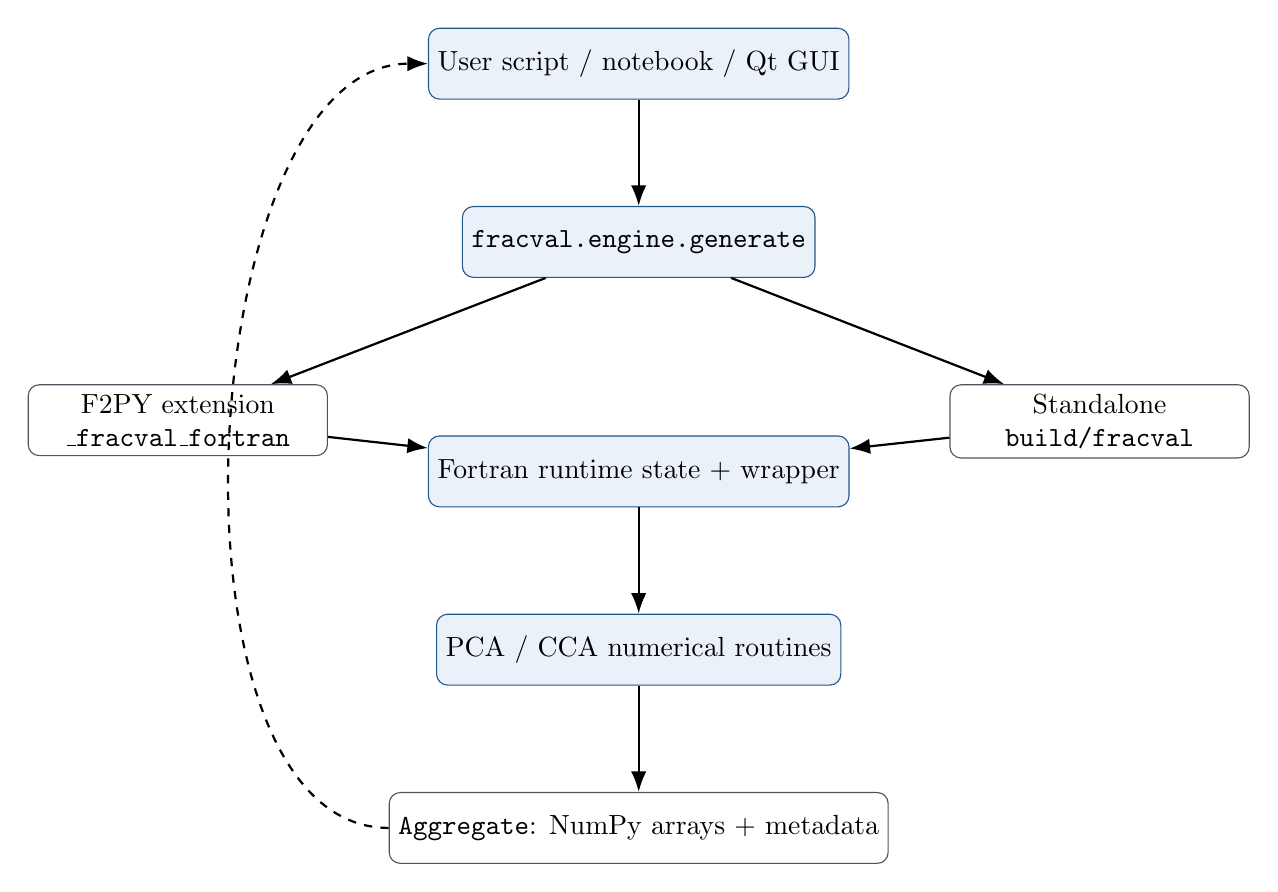
\begin{tikzpicture}[
  node distance=1.35cm and 1.7cm,
  box/.style={draw=FracBlue, rounded corners, fill=FracBlueLight, align=center, minimum width=3.8cm, minimum height=0.9cm},
  graybox/.style={draw=FracGray, rounded corners, align=center, minimum width=3.8cm, minimum height=0.9cm},
  arr/.style={-{Latex[length=2.6mm]}, thick}
]
  \node[box] (client) {User script / notebook / Qt GUI};
  \node[box, below=of client] (engine) {\code{fracval.engine.generate}};
  \node[graybox, below left=of engine] (extension) {F2PY extension\\\texttt{\_fracval\_fortran}};
  \node[graybox, below right=of engine] (executable) {Standalone\\\code{build/fracval}};
  \node[box, below=2.0cm of engine] (wrapper) {Fortran runtime state + wrapper};
  \node[box, below=of wrapper] (legacy) {PCA / CCA numerical routines};
  \node[graybox, below=of legacy] (result) {\code{Aggregate}: NumPy arrays + metadata};
  \draw[arr] (client) -- (engine);
  \draw[arr] (engine) -- (extension);
  \draw[arr] (engine) -- (executable);
  \draw[arr] (extension) -- (wrapper);
  \draw[arr] (executable) -- (wrapper);
  \draw[arr] (wrapper) -- (legacy);
  \draw[arr] (legacy) -- (result);
  \draw[arr, dashed] (result.west) .. controls +(-3,0) and +(-3,0) .. (client.west);
\end{tikzpicture}
\end{center}

\section{F2PY extension backend}

The preferred backend calls \code{fracval\_generate} in
\path{src/fracval_python_api.f90}. Inputs are scalar runtime values; outputs are
\(x,y,z,r\) arrays plus realized contact overlaps and status information.

The wrapper is marked thread-safe at the F2PY boundary so the generated C layer
releases the Python GIL while native Fortran runs. However, the underlying
Fortran modules use shared global state, so \path{engine.py} still serializes
extension calls with a process-local lock.

\section{Executable fallback}

The executable backend writes a temporary namelist, invokes the standalone
program, reads the produced DAT/contact files, and deletes the temporary
working directory. A custom executable may be supplied to \code{generate()} or
through the \code{FRACVAL\_EXECUTABLE} environment variable.

\section{Why both backends exist}

The extension is faster and cleaner for Python because it avoids temporary
files. The executable fallback is valuable for debugging, cross-checking, and
environments where building a Python extension is inconvenient. Regression
tests compare the two for fixed-seed cases.

\chapter{Testing and Validation}

\section{Core test command}

\begin{lstlisting}[language=bash]
make test PYTHON=python
\end{lstlisting}

This runs standalone Fortran cases plus Python/F2PY regression checks.

\section{What the tests cover}

The current suite checks:
\begin{itemize}
  \item runtime namelist execution;
  \item monodisperse radius behavior;
  \item polydisperse radius variation;
  \item fixed-seed F2PY reproducibility;
  \item F2PY versus standalone executable equivalence within output precision;
  \item \(N-1\) zero contact records in legacy no-overlap mode;
  \item fixed 5 percent overlap at intended contacts;
  \item bounded and varying statistical overlap;
  \item final pair geometry to detect unexpected overlapping pairs;
  \item visualization construction;
  \item configuration JSON and result-bundle round trips;
  \item runtime backend diagnostics.
\end{itemize}

\section{Qt tests}

After installing GUI dependencies:

\begin{lstlisting}[language=bash]
make qt-check PYTHON=python
make gui-test PYTHON=python
\end{lstlisting}

The GUI smoke test selects an available headless Qt platform plugin and
constructs the application without requiring a visible display.

\section{Debug Fortran build}

\begin{lstlisting}[language=bash]
make debug
\end{lstlisting}

This rebuilds with warnings, bounds/runtime checks, debug symbols, and
backtraces. Use it when changing numerical code.

\chapter{Extending FracVAL Safely}

\section{Python-only feature}

If a feature only analyzes, filters, visualizes, or exports an already-created
aggregate, implement it in Python. Add tests that create an \code{Aggregate}
or use a fixed-seed generated sample. There is no need to change the Fortran
core.

\section{Adding a new physical generation parameter}

A setting that affects placement should be propagated consistently:

\begin{enumerate}
  \item add runtime storage/default/validation to \path{src/Ctes.f90};
  \item modify the appropriate PCA/CCA routine;
  \item add the parameter to \path{src/fracval_python_api.f90};
  \item update \path{python/fracval/_fracval_fortran.pyf};
  \item add a field and validation to \code{FracVALConfig};
  \item pass it from \path{engine.py};
  \item include it in executable namelist generation;
  \item add GUI controls only after the API path works;
  \item add fixed-seed tests and update documentation.
\end{enumerate}

\begin{importantbox}
Do not implement scientific behavior exclusively in the GUI. The GUI should be
a client of the same generation API used by scripts and tests.
\end{importantbox}

\section{Adding a new export format}

If it is a text/data format, add a conversion method to \code{Aggregate} or a
helper in \path{io.py}, then expose it through the GUI only as a thin file-dialog
layer. Keep metadata/provenance explicit.

\section{Adding another visualization backend}

Keep \code{Aggregate} as the input boundary. A future VTK/PyVista/OpenGL viewer
can replace or complement Plotly without changing the Fortran or generation
API.

\section{Version-control guidance}

Do not commit platform-specific extension binaries, object files, module files,
or local virtual environments. The supplied \code{make clean} target removes
native build outputs. Keep fixed-seed regression cases in version control so
scientific changes can be compared deliberately.

\chapter{Troubleshooting}

\section{No backend is available}

Run:

\begin{lstlisting}[language=bash]
fracval-info
\end{lstlisting}

Then build one or both backends:

\begin{lstlisting}[language=bash]
make
make python-ext PYTHON=python
\end{lstlisting}

\section{\code{Could not find the Qt platform plugin "cocoa"}}

First ensure the same environment is used for install and launch:

\begin{lstlisting}[language=bash]
source .venv/bin/activate
which python
python -c "import PySide6; print(PySide6.__file__)"
fracval-qt-check
\end{lstlisting}

The runtime helper searches the active PySide6 installation and common Conda Qt
plugin layouts, then configures the plugin directory before Qt starts.

If PySide6 itself is incomplete, reinstall it in the active environment:

\begin{lstlisting}[language=bash]
python -m pip uninstall -y PySide6 PySide6_Addons PySide6_Essentials shiboken6
python -m pip install --no-cache-dir PySide6
\end{lstlisting}

\section{F2PY extension build fails}

Check:

\begin{lstlisting}[language=bash]
which python
python -c "import numpy; print(numpy.__version__)"
which gfortran
gfortran --version
\end{lstlisting}

Then clean and rebuild:

\begin{lstlisting}[language=bash]
make clean
make python-ext PYTHON=python
\end{lstlisting}

Because the extension ABI is Python/platform-specific, rebuild it after changing
to a different Python installation or architecture.

\section{Many \code{PC not able to continue} / restart messages}

A restart means the stochastic algorithm could not continue the current
construction while satisfying its geometry checks. Possible responses:
\begin{itemize}
  \item verify that \code{Df}, \code{kf}, size distribution, and overlap are reasonable for the intended model;
  \item increase \code{max\_attempts} for a legitimately difficult case;
  \item keep \code{Nsubcl\_perc=0.10} unless a known legacy case requires adjustment;
  \item reduce aggressive intended overlap and retest;
  \item run a debug build if behavior changed after code modifications.
\end{itemize}

Do not simply relax \code{tol\_ov} to force a physical overlap model.

\section{The GUI opens but generation fails}

Check the status/error dialog, then run the same configuration through Python
with a fixed seed. Scripted generation produces a more convenient exception for
logging and is easier to reproduce in a bug report.

\section{3-D rendering is slow}

Switch Display from Spheres to Centers or lower sphere resolution. Rendering
cost is separate from Fortran generation cost.

\chapter{Command and API Reference}

\section{Installed commands}

\begin{longtable}{p{0.31\textwidth}p{0.59\textwidth}}
\toprule
Command & Purpose \\
\midrule
\code{fracval-gui} & Launch native PySide6 desktop application. \\
\code{fracval-python} & Generate one aggregate from command-line Python arguments. \\
\code{fracval-info} & Report Python, package, extension and backend diagnostics. \\
\code{fracval-qt-check} & Report Qt/PySide6 plugin paths and platform availability. \\
\bottomrule
\end{longtable}

\section{Public Python functions}

\begin{longtable}{p{0.34\textwidth}p{0.56\textwidth}}
\toprule
Name & Purpose \\
\midrule
\code{generate(config, ...)} & Generate one aggregate. \\
\code{generate\_batch(count, config, ...)} & Return a list of aggregates. \\
\code{iter\_generate\_batch(count, config, ...)} & Stream aggregates one at a time. \\
\code{available\_backends()} & List currently usable generation backends. \\
\code{extension\_available()} & Test whether the F2PY extension imports. \\
\code{load\_data(path)} & Read a four-column native DAT file into NumPy. \\
\code{save\_bundle(aggregate, directory, ...)} & Save data, contacts, and metadata with a common stem. \\
\code{load\_bundle(metadata\_path)} & Reconstruct an Aggregate from a saved bundle. \\
\code{plot\_3d(...)} & Return an interactive Plotly 3-D figure. \\
\code{plot\_static(...)} & Return a Matplotlib 3-D figure. \\
\code{runtime\_info()} & Return environment diagnostics as a dictionary. \\
\bottomrule
\end{longtable}

\section{FracVALConfig fields}

\begin{longtable}{p{0.28\textwidth}p{0.18\textwidth}p{0.44\textwidth}}
\toprule
Field & Default & Meaning \\
\midrule
\endhead
\code{n} & 100 & primary-particle count \\
\code{df} & 1.79 & fractal dimension \\
\code{kf} & 1.40 & fractal prefactor \\
\code{rp\_g} & 15.0 & geometric mean radius \\
\code{rp\_gstd} & 1.0 & geometric radius standard deviation \\
\code{ext\_case} & 0 & legacy extreme-case flag \\
\code{nsubcl\_perc} & 0.10 & sub-cluster fraction \\
\code{tol\_ov} & \(10^{-6}\) & unintended-overlap numerical tolerance \\
\code{seed} & None & fixed seed or Python-selected fresh seed \\
\code{max\_attempts} & 250 & maximum construction restarts in extension path \\
\code{overlap\_mode} & none & none, fixed, or statistical \\
\code{overlap\_fraction} & 0.0 & fixed intended-contact overlap \\
\code{overlap\_mean} & 0.05 & statistical mean \\
\code{overlap\_std} & 0.02 & statistical standard deviation \\
\code{overlap\_max} & 0.12 & statistical hard upper bound \\
\bottomrule
\end{longtable}

\section{ViewerAppearance fields}

\begin{longtable}{p{0.29\textwidth}p{0.20\textwidth}p{0.41\textwidth}}
\toprule
Field & Default & Meaning \\
\midrule
\code{color\_mode} & solid & solid or radius-based coloring \\
\code{particle\_color} & \#4C78A8 & solid particle color \\
\code{colorscale} & Viridis & Plotly radius color scale \\
\code{opacity} & 0.96 & particle opacity \\
\code{shininess} & 0.55 & specular/gloss appearance in sphere mode \\
\code{background\_color} & \#FFFFFF & scene/page background \\
\code{show\_axes} & false & show XYZ axes/grid \\
\code{show\_colorbar} & false & show radius legend when radius-colored \\
\code{show\_title} & true & show figure title \\
\bottomrule
\end{longtable}

\chapter{Worked Python Examples}

The following files are included under \path{examples/python/}. They are meant
to be copied and adapted rather than treated as hidden framework code.

\section{Basic generation and bundle export}
\lstinputlisting[language=Python]{../examples/python/01_basic_generate.py}

\section{Overlap comparison}
\lstinputlisting[language=Python]{../examples/python/03_overlap_models.py}

\section{Batch generation}
\lstinputlisting[language=Python]{../examples/python/04_batch_and_export.py}

\section{Parameter sweep}
\lstinputlisting[language=Python]{../examples/python/05_parameter_sweep.py}

\appendix
\chapter{Makefile Target Reference}

\begin{longtable}{p{0.32\textwidth}p{0.58\textwidth}}
\toprule
Target & Action \\
\midrule
\code{make} & Build \path{build/fracval}. \\
\code{make run} & Run default \path{fracval.in}. \\
\code{make run INPUT=x} & Run a named input file. \\
\code{make install} & Install editable Python package and F2PY extension. \\
\code{make install-gui} & Install GUI dependencies and extension. \\
\code{make info} & Print Python/backend diagnostics. \\
\code{make python-ext} & Build in-memory Fortran extension. \\
\code{make fortran-test} & Run standalone cases. \\
\code{make python-test} & Run Python scientific/visualization tests. \\
\code{make test} & Run Fortran and Python tests. \\
\code{make qt-check} & Diagnose Qt platform plugins. \\
\code{make gui-test} & Headless Qt construction smoke test. \\
\code{make gui} & Launch the native desktop application. \\
\code{make plot-test} & Exercise static and interactive plotting. \\
\code{make debug} & Rebuild Fortran with runtime checking. \\
\code{make docs} & Compile this LaTeX manual to PDF. \\
\code{make clean} & Remove native build artifacts. \\
\bottomrule
\end{longtable}

\chapter{Recommended Scientific Workflow Checklist}

\begin{enumerate}
  \item Record \code{N}, \code{Df}, \code{kf}, particle-size distribution, overlap model, and seed.
  \item Use a fixed seed while developing or validating a case.
  \item Run \code{make test} after modifying the Fortran/Python interface.
  \item Save aggregate metadata or a bundle, not only a DAT file.
  \item Keep overlap distinct from \code{tol\_ov}.
  \item Use the F2PY backend for normal Python work and the executable backend as a useful cross-check.
  \item For parameter sweeps, log failed seeds/configurations instead of silently skipping them.
  \item Use multiprocessing rather than threads for process-level generation parallelism.
  \item Rebuild the native extension after changing Python versions or architectures.
  \item Keep the GUI as an interface layer; add reusable scientific functionality to the public Python API.
\end{enumerate}

\begin{tipbox}
The fastest route for a new user is: create a virtual environment, run
\code{make install-gui PYTHON=python}, run \code{make}, verify with
\code{fracval-info}, and then use either \code{fracval-gui} or the public
\code{fracval} Python API. The full project is designed so those two workflows
share the same Fortran generator.
\end{tipbox}

\end{document}
